%%%%%%%%%%%%%%%%%%%%%%%%%%%%%% -*- Mode: Latex -*- %%%%%%%%%%%%%%%%%%%%%%%%%%%%
%% project.tex -- 
%% Author          : Philip Johnson
%% Created On      : Tue Mar 31 11:44:58 2009
%% Last Modified By: Philip Johnson
%% Last Modified On: Sat Apr 18 11:54:34 2009
%% RCS: $Id$
%%%%%%%%%%%%%%%%%%%%%%%%%%%%%%%%%%%%%%%%%%%%%%%%%%%%%%%%%%%%%%%%%%%%%%%%%%%%%%%
%%   Copyright (C) 2009 
%%%%%%%%%%%%%%%%%%%%%%%%%%%%%%%%%%%%%%%%%%%%%%%%%%%%%%%%%%%%%%%%%%%%%%%%%%%%%%%
%% 

\pagenumbering{arabic}
\renewcommand{\thepage} {C--\arabic{page}}

\renewcommand{\thesection} {C.\arabic{section}}
\setcounter{section}{0}

\section{Project Description}

\subsection{Project Vision, Goals, Objectives, and Outcomes}

{\em Section requirements: Describe the CT-centric vision, goals,
objectives, and anticipated outcomes of the proposed project. Clearly
indicate how they will contribute to realization of the three CPATH program
goals: (1) contribute to the development of a globally competitive
U.S. workforce with CT competencies essential to U.S. leadership in the
global innovation enterprise; (2) increase the number of students
developing CT competencies by infusing CT learning opportunities into
undergraduate education in the core computing - computer and information
science and engineering - disciplines, and in other fields of study; and,
(3) demonstrate transformative CT-focused undergraduate education models
that are replicable across a variety of institutions.

Evaluation criteria: Assess the potential of the proposed project and the
likelihood that it will contribute in significant ways to realization of
the CPATH program goals.
}
\bigskip

Jeannette Wing has written, ``Computational thinking involves solving
problems, designing systems, and understanding human behavior, by drawing
on the concepts fundamental to computer science'' \citep{Wing06}.  In her
presentation ``Computational Thinking and Thinking About Computation'',
Wing refines her view of these fundamental computer science concepts in terms of 
the ``Two As'': Abstraction and Automation.  Activities
related to the first ``A'' include: choosing the right abstractions, operating
at multiple levels of abstraction, and defining relationships between
abstractions.  Activities related to the second ``A'' involve mechanizing the
first A via precise notations and models.  In essence, automation amplifies
the power of abstraction.  Computational thinking, from this perspective,
involves the correct choice of abstraction combined with the correct choice
of automation.

The vision of this proposal is to develop and institutionalize a new
approach to computational thinking where abstraction and automation combine
to transform the use of {\em empirical thinking} in software development.
We call this approach ``empirical computational thinking'', or \eCT.

To introduce our approach, we must first address what is meant by
empirical thinking.  The term ``empirical'' is variously defined as
``derived from experiment and observation rather than theory''; ``evidence
or consequences observable by the senses''; and ``capable of being verified
or disproved by observation or experiment.''

Given these definitions, it is clear that some degree of empirical thinking
is already commonplace in software development.  For example, beginning
programmers use empirical thinking when they ``observe'' the output of the
compiler to learn how to write syntactically correct programs.  Beginners
also tend to make extensive use of ``experimentation'': they execute their
program with example data, compare the actual behavior to what they expect,
then make modifications until the observed behavior matches their
expectations.

These examples of empirical thinking, while typical for beginning
programmers, do not scale well because they lack both abstraction and
automation. Thus, they fail to constitute the kind of computational
thinking of interest to the CPATH program, and they fail as well to be
\eCT.

One would hope that as students progress into more advanced software
development courses, the curriculum would scale in at least two
ways. First, the complexity, size, and number of people involved in a
software development project would scale upwards.  Second, the level of
abstraction and automation in their empirical thinking would scale
commensurately. Unfortunately, while advanced software development courses
certainly require students to develop significantly more sophisticated
systems than their introductory counterparts, the use of empirical thinking
remains mostly non-abstract and non-automated.  The principle computational
support for advanced programming classes is an integrated development
environment such as Eclipse or Visual Studio. While this is a significant
advance over vanilla text editors, such IDEs provide relatively little in
the way of abstraction or automation for empirical thinking about the
products and processes of software development.

Supporting abstraction in empirical thinking for software development
generally means creating quantitative models for important development
concepts.  For example, test quality is an important concept that is
commonly emphasized in advanced software development courses.  One
quantitative model for test quality is line-level test coverage, which is
generally expressed as the percentage of source lines of code in the
software exercised by the test cases.  Another important concept is
complexity, and quantitative models such as afferent and efferent coupling
or cyclomatic complexity provide abstract, empirical representations for
this concept.  Even ``agile'' concepts such as ``commit early, commit
often'' or ``collective code ownership'' can support abstract, empirical
models. For example, ``commit early'' can be modeled as the percentage of
files in the system that are committed within a certain number of days of
their creation.  ``Collective code ownership'' can be modeled by the
percentage of files in the system that have been edited by every member of
the development team.

Supporting automation for these abstractions of empirical thinking for
software development means tool support for collecting, analyzing,
disseminating, and interpreting these abstractions.  For example, an
automated process can run once a day and calculate the current coverage and
complexity values for the system.  These values can be made available to
the user by a web application. Alternatively, email ``alerts'' can be sent
to the developers when coverage crosses a threshold and becomes too low, or
coupling crosses a threshold and becomes too high.  Plugins to development
tools like IDEs can collect information on what files are edited when in
order to determine the age of a file when it is first committed, or the
degree of collective editing on the file.  

Thus, our vision for \eCT\ includes programming as an activity that is rich
in automated, abstract representations of development processes and
products, made available conveniently and appropriately for observation and
reflection by the programmers.  It also includes education in the analytic
capabilities required to effectively interpret these representations, to
understand their limitations as representations of reality, to know when to
take action based upon them and what kind of action is warranted.

The goal of this research is to explore, evaluate, and institutionalize
techniques and technologies for \eCT, building upon research and education
we have worked on over the past ten years in empirically-based software
engineering.  For example, we recently performed an initial evaluation of a
novel system and associated curriculum we developed called the ``Software
Intensive Care Unit'' \citep{csdl2-09-02}.  In this approach, sensors
attached to development tools automatically collect student process and
product data and abstract it into a set of ten ``vital signs'' that provide
an empirical basis for students to assess the ``health'' of their ongoing
projects.  The Software ICU is an example of \eCT, as it supports both
automated and abstract empirical thinking about the current state and past
history of both their projects and their group processes.  Our curriculum
materials taught students how to introduce the Software ICU data collection
sensors into their laptop development environments, how to obtain the
analyses, and how to interpret the results.

While we are excited by the potential of our own prior work in \eCT, there
are other research and educational initiatives that conform to our broader
vision for \eCT.  Our goal is to organize and develop a constellation of
approaches to \eCT\ and build a body of knowledge that enables future
researchers and educators to understand the comparative strengths and
weaknesses of the various approaches and to create innovative new
approaches to \eCT\ that go synthesize and/or extend beyond any of the
present day capabilities.

To achieve this goal, we will pursue three concrete objectives, organized
according to the three years of this grant.  

First, we will perform a study during the 2009-2010 academic year at the
University of Hawaii in which we will validate and extend the findings from
our initial case study of the Software ICU during 2008.  We will also begin
trial use of a second approach to \eCT\ we have developed called Devcathlon. 
Finally, we will begin development of a common evaluation framework for \eCT\ that
can be used to 

Second, we will partner with other academic institutions and departments
during the 2010-2011 academic year to gain insight into the issues that
occur when integrating empirical thinking into other advanced software
development courses.  In addition, we will begin exploring the issues
involved in adapting these initial materials both downward (into more
elementary curriculum); upward (into post-scholastic, professsional
settings); and outward (into related disciplines such as engineering or
information technology).

Third, we will use the data gathered and the collaborations formed during
the first two years to form an open source consortium to further spread the
use of abstract, automated empirical thinking.  This consortium will itself
be transformative in that it will combine open source technologies (such as
the Software ICU and Devcathlon) with open source curriculum materials
(which facilitate the introduction of the materials) with open source data
(results from the application of these technologies and pedagogies, which
can be used to guide future evolution of these approach).  The goal is to
go far beyond web site publication and create a social network of students
and educators interested in advancing the use of empirical thinking in
software development

Our vision, goal, and objectives are designed to produce outcomes that
directly support the goals of the CPATH program.  First, establishing
automated, abstract empirical thinking as an integral component of software
development courses can significantly improve the competitiveness of our
software engineering workforce by giving them facility with a powerful tool
for computational thinking.  Second, our approach begins by infusing a new,
empirical form of computational thinking into the advanced software
development curriculum and then propogates it downward, upward, and
outward.  Third, we will collect data and experiences on the effectiveness
of this approach across a variety of institutions and pedagogical models.

\subsection{Intellectual Basis/Related Work}

{\em Section requirements: Describe the intellectual basis for the project
and discuss related prior work.  Include a review of the research
literature relevant to the project and provide corresponding references.

Evaluation Criteria: Assess the proposed intellectual contribution, and the
potential for dissemination and adaptation in the national community.}
\bigskip

\subsubsection{Research from the empirical software engineering community}

As noted above, empirical thinking occurs naturally in software development
activities.  There is a well-established research community focusing on the
promulgation and advancement of empirical techniques in software
development.  Organizations such as the International Software Engineering
Research Network (ISERN), journals such as Empirical Software Engineering,
and conferences such as the International Symposium on Empirical Software
Engineering and Measurement all provide active forums for the role of
empirical thinking in software development.

Unfortunately, review of these forums indicates that the role of empirical
thinking in the software development curriculum receives relatively little
attention.  For example, in the 328 articles published in Empirical
Software Engineering from 2002 to 2008, we found only one article that
focused explicitly on the use of empirical techniques as part of software
development pedagogy \citep{Pfahl03}.  Through review of the other
articles, we found that while students are frequently employed in empirical
research, the goal of their participation is to support the testing of a
research hypothesis unrelated to classroom pedagogy.  For example,
\cite{Babar08} used students to support a controlled study of the
differences between distributed and face-to-face meetings for software
architecture evaluation.  \cite{Carver06} used students as subjects to test
an approach for helping novice programmers learn software inspection
techniques more quickly.  \cite{Host00} performed a study in which students
were used to determine if the data collected from students differs from
data collected from professionals.

The Dagstuhl Workshop on Empirical Software Engineering Issues
\citep{Basili06} contained a track on educational issues, but a primary
focus was the use of students as subjects for empirical experimentation.

The Empirical Studies of Programmers workshop series (now discontinued)
focused on the use of empirical technique to understand programmer
behavior, rather than teaching students how to use empirical thinking to
affect their own behavior.  This emphasis is shared to a great extent by
the Journal of Educational Resources in Computing, now renamed ACM
Transactions on Computing Education.

The Empirical Software Engineering and Measurement conference series has
provided a forum for a variety of applications of empirical techniques,
including those for testing and analysis, coordination and communication,
estimation, modeling and architecture, inspections, defect classification,
and fault-prone module prediction.  We found only one paper that focused
explicitly on the introduction of empirical techniques into the classroom
setting was \citep{csdl2-03-12}.

Finally, we have directly solicited information about their classroom
pedagocy from the empirical software engineering community using internal
mailing lists and personal contacts. We found evidence that courses at a
variety of universities include material related to empirical techniques,
including: University of Rome/Tor Vergata; Mississippi State University;
Norwegian University of Science and Technology; University of Insubria;
University of Southern California; University of Maryland; University of
Bari; University of Sheffield; Seattle University; University of Virginia;
University of Ottawa; Keele University; University of Karlsruhe;
Polytechnical University of Madrid; University of Calgary; and University
of Toronto.  However, the material was generally related to using students
as subjects (undergraduate level) or the teaching of experimental
methodologies (graduate level).  One exception is the University of
Southern California, where students gather empirical data for abstraction
using the COCOMO cost modeling system to estimate effort and time for their
projects.

\subsubsection{Research in the software engineering education community}

The previous section demonstrates that the empirical software engineering
community does not (yet) focus on the pedagogy of empirical thinking. Fortunately, 
there is more evidence of interest in this approach in the software education 
research community.

In 1995, Watts Humphrey authored {\em A Discipline for Software
Engineering}, a ground-breaking text that adapted organizational-level
software measurement and analysis techniques to the individual developer
along with a one semester curriculum. These techniques are called the
Personal Software Process (PSP), and form the basis for the Team Software
Process (TSP), which extends the method to groups of developers. 

The PSP is the best known and most widespread approach to empirical
thinking in the advanced software development curriculum.  The approach
requires students to develop a series of software projects, typically six
to eight during a single semester.  Both process and product measures are
gathered about each project, and the measurements become increasingly
detailed as the semester proceeds. After the first three projects are
completed, the students can use the completed projects as historical data
to support quality improvement (by identifying repeated types of defects)
and estimation (through simple linear regression).  The PSP and TSP enjoy
strong support from the Software Engineering Institute, which has published
a number of case studies indicating success in a classroom setting and
which sponsors a yearly symposium to publicize academic and industry
experiences.  The PSP/TSP enable support for very basic levels of
abstraction and automation of empirical thinking. For example, the PSP
Dashboard is a tool that allows students to enter the data they collect and
which will automate the calculation of regression lines.

Conn developed a metrics-based software engineering course called the 
IS Integrated Capstone Project \cite{Conn04}.  The metrics were closely aligned
with the PSP/TSP format, though some of the process constraints were relaxed. 

Robillard designed a project-based course in which students were required
to fill out logs that specified the time spent on various activities
\cite{Robillard98}.  However, minimal abstraction and no automation was supported.

One recent research effort shows how abstract and automated empirical
thinking can be used in introductory programming courses. The Retina system
automatically collects editing and compilation data on beginning
programmers, which it then abstracts using a recommendation and suggestion
subsystem \cite{Murphy09}.  Retina can notice, for example, when a student
is getting many more errors per compilation than other students in the
class, and recommend that the student might want to break the work down
into smaller pieces.  Retina is designed around the needs of introductory
programming classes, where students typically work alone, do not use a wide
range of development tools, and a significant amount of energy is devoted
to obtaining a syntactically correct program.  Nevertheless, it
demonstrates that there is significant potential for the use of abstract,
automated, empirical thinking throughout the software development
curriculum.

\subsubsection{From empirical to scientific and evidence-based thinking}

Integrating computational thinking concepts (automation and abstraction)
with empirical thinking has the potential to transform and improve the
software development curriculum in profound ways. One of the most important
benefits of introducing empirical thinking is that it is a necessary
precursor for scientific and evidence-based thinking in software
development.

One of the most eloquent descriptions of the difference between empirical
and scientific thinking is provided by John Dewey \citep{Dewey10}.  In his
chapter ``Empirical and Scientific Thinking'', Dewey begins by noting that
empirical thinking, which is based purely on observation, has been used by
humans throughout history as a way of understanding through association.
For example, upon repeatedly noticing that when the sky is lowering upon
sunset, rain follows the next day, one might form the ``conclusion'' that
if the sky is lowering at sunset, rain will follow.  He follows this with a
discussion of the danger of confusing correlation with causality, and
introduces the scientific method as a way of addressing this problem.  From
Dewey's point of view, the scientific method involves active
experimentation under controlled or semi-controlled conditions (as opposed
to passive observation) and the formation of testable theories that
introduce causal mechanisms (for which evidence can be gathered to support,
refute, or refine).  A major focus of the empirical software engineering
community is to develop experimental techniques applicable to software
development practice that replace simple observation with more controlled,
hypothesis-driven analysis.

A related effort is the application of evidence-based medical research
techniques to software development \citep{Kitchenham04,Kitchenham04a},
which involves a five step method: (1) Convert the need for information
[about a software engineering practice] into an answerable question; (2)
Track down the best evidence available for answering the question; (3)
Critically appraise that evidence using systematic review for its validity
(closeness to the truth), impact (size of the effect), and applicability
(usefulness in software development practice); (4) Integrate the critical
appraisal with current software engineering knowledge and stakeholder
values [to support decision-making]; (5) Evaluate the effectiveness and
efficiency in applying Steps 1-4 and seek ways to improve them for next
time.  While promising, application of systematic reviews and the
integration of empirical software engineering data from multiple sources
has been found to be challenging \citep{Jedlitschka04}.  Evidence-based
software engineering is also a topic of interest to the empirical software
engineering community.

%% GQM??

\subsubsection{Conclusions}

From review of this related work, we can see that the empirical software
development method with the longest history and most industrial support is
the PSP/TSP.  However, it enjoys relatively limited levels of abstraction
and automation.  It is also purely observational in nature and does not
integrate scientific or evidence-based methods.

We can also see that there is a tremendous opportunity for synergy with the
empirical software engineering community by collaborating on development of
curriculum that engages students as direct participants in empirical
observation and analysis.  The University of Southern California has
demonstrated that this is possible.

There is also evidence that abstract and automated empirical thinking can
be applied outside the confines of advanced software development courses.
The Retina system shows how even introductory courses can benefit.


\subsection{Current State}

{\em Section requirements: Provide a current assessment of undergraduate
education in the relevant participating organizations.  Describe prior
pilot programs or planning activities conducted to date, if any, and their
outcomes.  Where appropriate, provide institutional data to document the
current environment by uploading data into the Supplementary Docs section
in FastLane.

Evaluation Criteria: Evaluate the readiness of the participating
organizations to undertake the proposed work.  Do the proposers demonstrate
a clear understanding of the current state of undergraduate computing
education within the nation, within the participating organizations, and
within the domain of focus for the proposed project?  If data are provided,
do they support the proposing team's assessment?}
\bigskip

For over ten years, we have been exploring empirical software engineering
techniques and their applications in the classroom setting as part of our
research in the Collaborative Software Development Laboratory at the
University of Hawaii.  This section summarizes our prior studies and the
current state of practice in our institution.

{\bf PSP.} Beginning in the late 1990's, we instituted the use
of the Personal Software Process in both undergraduate and graduate
software engineering courses.  While our outcomes were quite positive and
in line with the data gathered by the Software Engineering Institute, we
were concerned by the possibility of data quality problems and the lack of
automation.  To investigate the first question, we undertook a study of PSP
data quality which found that manual collection and analysis could result
in data quality problems that could effect the outcomes and interpretation
of the data \citep{csdl-98-13,csdl-98-11}.  To investigate the second question, we
implemented extensive tool support for PSP/TSP style of data collection and
analysis \citep{csdl2-00-03}, but still found the overhead to be
substantial\citep{csdl2-01-12}. 

{\bf Hackystat.} In 2001, we initiated a research project called Hackystat
\citep{csdl2-06-06,csdl2-04-11,csdl2-02-07}, one of whose goals is to
support abstract and automated empirical thinking in the classroom setting
in a manner different from the PSP/TSP.  To accomplish this, we changed the
types of data collected and the nature of the analyses and interpretations
provided by the framework.  For example, in the PSP/TSP (as well as other
approaches like COCOMO), data on completed projects is used to make
predictions about future, as-yet-unstarted projects. Hackystat
instead uses ``sensors'' attached to development tools to automatically and
unobtrusively collect fine-grained process and product data. Analyses on
this data are intended for direct feedback into the current system under
development, not for use in future system planning.

For the past five years, Hackystat has been an integral part of the
University of Hawaii software engineering curriculum at both the
undergraduate and graduate levels.  We performed case study experiments in
2003 \citep{csdl2-03-12,csdl2-03-13}, 2006 \citep{csdl2-07-02}, and 2008
\citep{csdl2-09-02,csdl2-09-03} to assess the classroom impact and
effectiveness of the system in supported automated and abstract empirical
thinking.  Each case study collected both quantitative and qualitative data
that motivated extensive redesign and improvement of the system, which we
evaluated in the subsequent case study. While the details of evaluation
differed in the three studies, in all cases we were generally concerned
with three issues: (1) What was the perceived overhead of the system? In
other words, how well does the system provide automation?  (2) What was the
perceived utility of the system? In other words, how well does the system
provide abstraction?  (3) How well will the system apply to
``professional'' settings?  In other words, to what extent does the
empirical thinking promoted by this system feel relevant and useful in the
long term?

These case studies generated a great deal of useful data that has directly
influenced the course of our research and educational practice. For
example, the 2003 experiment provided data indicating that sensor
installation was perceived as a significant barrier to use. From the \eCT\
perspective, this is an example of a failure of the system to provide
sufficient automation.  The 2006 experiment provided data indicating that
students had difficulties interpreting the trends in data and understanding
when the data indicated the need for a change in behavior.  From the \eCT\
perspective, this is an example of a failure of the system to provide
sufficient abstraction.  In all three case studies, students have raised
concerns about privacy issues.  This is an example of a challenge and
potential limitation of this approach to support empirical thinking.

{\bf Software ICU.}  In 2008, we performed an initial case study evaluation 
of a new approach to teaching \eCT\ concepts.  In this approach, we frame 
\eCT\ within the metaphor of a medical intensive care unit (ICU). 

Medical intensive care units feature automatic and continuous monitoring of
patient vital signs.  The four fundamental medical vital signs are
temperature, heart rate, blood pressure and respiration.  Other vital signs
may be monitored depending upon the particulars of a patient condition.
Vital signs have a ``normal range of behavior'', and the monitoring unit
can raise an alarm when any of the patient's vital signs departs from its
normal range of behavior.

Vital signs are interesting because: (a) in a healthy patient, they are
normal or improving; (b) change in one vital sign may or may not be
significant; (c) change in multiple vital signs is almost certainly
significant, particularly if more than one are outside their normal range.

The Software ICU translates ``health'', ``ital signs'', ``normal range''
and the ICU monitoring user interface into terms useful to students and their
software development projects.

We defined a healthy development project as satisfying three high-level
characteristics: high efficiency (software development proceeds ``as fast
as possible, but no faster''); high effectiveness (effort is focused on the
most important issues, with minimal rework); and high quality (software
satisfies user needs; software can be easily installed, adapted, and
maintained).

We then presented a set of simple practices that, if followed, we claimed
would improve the health of their projects.  These included: everyone works
consistently; everyone contributes equally; code is committed consistently;
progress is regular; quality remains high; no last minute rush to finish.
These development practices are analogous to life-style behaviors like
``eat right'', ``get enough sleep'' and ``exercise regularly'' that
generally facilitate (but, of course, do not guarantee) good health in a
patient.

Next, we presented nine software vital signs: coverage, complexity,
coupling, churn, builds, commits, unit tests, size, and dev time. Through a
combination of Hackystat sensors and the Hudson continuous integration
system, these nine vital signs could be automatically and continuously
collected for their projects.

For each software vital sign, we then presented its normal range of
behavior.  For example, for the coupling vital sign to be considered
healthy, its current value should be above 90\% and the trend in
coverage over time should be stable or increasing.  For the commit vital
sign to be considered normal, at least 50\% of the team members should have
committed, and there should be commits on at least 50\% of the days in the
project interval.  For one of the vital signs, size, we stated that
there is no simple way of assessing its normal range of behavior, though
it still provides some value in understanding project health.

Unlike a medical ICU, where there is literally hundreds of years of medical
research establishing both the importance of the four fundamental vital
signs and their normal range of behaviors, no such consensus exists in
software engineering on what would constitute ``fundamental'' software
vital signs or their normal range of behavior.  Thus, our selection of
software vital signs and their normal range of behaviors are actually
research hypotheses.  We designed a case study to elicit evidence
regarding the appropriateness of these vital signs and our proposed normal
range of behaviors.

Finally, we presented the user interface to the Software ICU. A portion of
this user interface appears in Figure \ref{fig:sicu}.

\begin{figure*}[ht]
  \center
  \includegraphics[width=0.8\textwidth]{portfolio-2008.eps}
  \caption{An example Software ICU display}
  \label{fig:sicu}
\end{figure*} 

Each row in the Software ICU interface provides information about one
software project.  Each column presents information about one vital
sign. Similar to the medical ICU, the software ICU presents both the most
recent numeric value as well as the recent trend in value for each vital
sign.  The normal range of behavior is represented by independently
coloring the trend line and the most recent value as green, yellow, or red
depending upon whether the value was healthy, unstable, or unhealthy.

The measurements underlying the Software ICU were collected automatically
through two mechanisms. First, the students installed Hackystat sensors
into their IDE (Eclipse) and build system (Ant) which sent process
metrics regarding their development activities.  Second, their projects
used the Hudson system to perform continuous integration, which meant that
after each commit of their code, the system would be automatically built
and tested.  The Hudson system was also configured to automatically gather
certain product metrics such as coverage, coupling, and complexity.

{\bf Devcathlon.} A current active research and development project involves
the creation of an environment in which \eCT\ principles are embedded within
a game environment.  Unlike other software development games which rely on
simulation of developer activities \cite{simSE}, Devcathlon is designed
around the use of actual data collected from students as they develop
software.  Students can form teams and play matches against each other.
Matches are based upon ``events'' which reward teams for appropriate
software development behaviors, such as ``commit early, commit often'',
``keep the coverage high'', and ``don't break the build''.

As of Spring, 2009, Devcathlon is under active development and we expect to
have an initial release for evaluation by Fall of 2009.


\subsection{Implementation Plan}
\label{sec:implementation}

{\em Section requirements: Describe in detail the CT-centric activities to
be undertaken to realize the project vision, goals, objectives and
anticipated outcomes.

Define, or describe how the proposing team will attempt to define, the core
computing concepts, methods, technologies and tools to be integrated into
promising new undergraduate education models.  Describe your plans to
identify and implement effective strategies to develop and assess CT
competencies in the relevant learning communities.  Identify the
stakeholder cohort, e.g. K-20 administrators, faculty, teachers, students,
etc., that will participate in and/or benefit from the activities. If
relevant, describe how change will be effected and sustained in the
participating organizations.

Describe project milestones in the context of a project timeline and
identify responsible parties and expected outcomes for each milestone.
Summarize this information in a figure that you upload into the
Supplementary Docs section in FastLane.

Describe how project outputs and outcomes will be disseminated to the
relevant stakeholder groups and to the national community and if relevant,
how project resources will be made available to others to adopt or
adapt. Identify proactive measures to find and support adopters of
promising models and/or practices. Describe plans for outreach to other
groups or interested institutions that will take place during the project.

Evaluation criteria: Evaluate the soundness of the proposed implementation
plan.  Determine the degree to which individuals from CISE disciplines are
engaged in the project, both in the leadership team and in the project as a
whole.  Assess the quality of the proposed dissemination activities.
}
\bigskip

Our implementation plan is comprised of several functional activities to be
distributed across the three years of the project.

{\bf Common \eCT\ Evaluation Framework development.}  A primary objective
of this project is to develop a framework for evaluation of \eCT\
initiatives.  The goal of this evaluation framework is to elicit useful
information concerning the ways in which a particular approach to \eCT\
provides for empirical, automated, and abstract thinking. Figure
\ref{fig:cef} provides an overview of the framework components.

\begin{figure}[!ht]
\begin{tabular}{|p{1in}|p{5in}|} \hline
{\bf Component} & {\bf Description}  \\ \hline

Student \newline Demographics & What are the required or desirable characteristics of the
student population that appear to make them suitable to this form of
\eCT? What kinds of prerequisite skills or technical background does this
form of \eCT\ presuppose?  
\\ \hline

Curriculum \newline Integration & 
Which course or courses are best suited to this form of
\eCT: introductory, intermediate, or advanced computer
programming? How does the \eCT\ experience integrate into the
chosen course: a stand-alone course (PSP/TSP), a ``mixin'' to an
existing course (Software ICU), or a short, self-contained ``module''?
\\ \hline

Empiricism & What types of observations are made by this form of \eCT? Are
they qualitative, quantitative, or some combination?  When are the
observations made?  What are the potential sources of error in these
observations? If there is the potential for error, can observations be
triangulated and/or cross-validated? What is the potential for measurement
dysfunction? What is the overhead on students and teachers to make these
observations?  
\\ \hline

Abstraction & Into what representations are the observations abstracted?
When are these abstractions made?  Is abstraction generation
student-controlled or teacher-controlled?  How are the results of
abstraction communicated to students?  Is this communication ``pull-based''
(i.e. students must manually request them), ``push-based'' (i.e. results
are sent to students via email, twitter, IM, etc.), or some combination?
What is the overhead on students and teachers to make these abstractions? 
\\ \hline

Automation & What forms of automation are used, if any, to: (a) collect
observations; (b) generate abstractions from the observations; (c)
visualize abstractions; (d) disseminate abstractions; (e) validate
abstractions?  What kinds of failure are possible with each type of
automation?  What is the overhead involved with setting up and maintaining
the automation?  What are the technical and infrastructure prerequisites
for employing the automation?
\\ \hline

Learning \newline outcomes & What are the intended learning outcomes from this form
of \eCT: what knowledge will students have; what skills will they have
assimilated; and what attitudes should this form of \eCT\ foster?  How can
these learning outcomes be measured as part of the \eCT\ curriculum
materials? 
\\ \hline

Outcome \newline data & What qualitative and quantitative data can be made
public after each instantiation of this form of \eCT? What kinds of
contextual information can be associated with this data in order to make it
more meaningful and amenable to meta-analysis and data mining, without
compromising privacy and confidentiality?  
\\ \hline


\end{tabular} 
\caption{Evaluation Framework Components}
\label{fig:cef}
\end{figure}

The Framework elicits information regarding six key aspects of an \eCT\
initiative: student demographics, curriculum integration, empiricism,
abstraction, automation, learning outcomes, and outcome data.  The
structure of this framework, and the questions we pursue within each area,
are based upon our prior \eCT\ experiences starting with the PSP and up to
our current evaluation of the Software ICU.

Addressing the questions in the Framework provides a good basis for
understanding the design trade-offs inherent in any \eCT\ effort.  For
example, the PSP sacrifices some potential forms of automated data
collection (i.e. time and defects) in order to support certain kinds of
abstraction (effort and quality estimation models).  Retina sacrifices many
kinds of empirical observations in order to address the limited programming
capabilities of novice programmers.

The Framework also illuminates opportunities for synergy between
initiatives and/or adaptation of innovations from one approach to another.
For example, PSP abstractions are mainly focussed on project planning
improvements through a historical database of past project data. The PSP
provides empirical techniques that enable you, based on your prior
performance, to make predictions about future project end dates and
required resources.  However, let's say that you have a team with
suboptimal behaviors.  In some sense, the PSP can even codify these
behaviors, as the team might get simply get better at predicting their
suboptimal performance.  The Software ICU, on the other hand, focuses purely 
on improving behavior without providing insight into the ``goal line''.  
Combining the two has the potential to address the weaknesses in both. 

The development of the Common \eCT\ Evaluation Framework will be ongoing
throughout the project.  During the first year of the project,
framework-related activities will consist of simply collecting information
about the ways in which currently known \eCT\ initiatives (such as PSP/TSP,
Software ICU, Devcathlon, SimSE, and Retina) address these issues.   We expect to 
refine the types of questions we ask and the way we capture the data as
part of the first year's activity. The result of this initial phase of data
gathering will form our ``baseline''. 

In subsequent years, we will use this baseline data to help push the \eCT\
community forward along two dimensions. First, the baseline should help us
establish more consistent, higher quality evaluation mechanisms. For
example, if one group has developed a particularly good instrument for
assessing student opinion, then the baseline can make this apparent and
help spread its use to other organizations.  Second, the baseline can
help assess attempts at synergy.  For example, it could help understand what 
new problems might arise from a composite PSP/TSP/Software ICU approach. 
It can reveal new opportunities, such as the possibility of adapting the 
Retina recommendation for use in advanced computer programming classes. 
Finally, it help reveal opportunities for transfer of insight. For example, 
both SimSE and the PSP/TSP have been evaluated in multiple university settings, 
while the Software ICU has not. 

On the other hand, it is not our goal for the framework to enable ``apples
to apples'' comparisons, such as ``Students using PSP/TSP learn more than
students using Retina'', or ``The Software ICU provides better abstractions
than Retina''.  We believe that the context, demographics, and goals of the
current \eCT\ initiatives are much too diverse those kinds of comparisons
to be valid or have value.


{\bf UH \eCT\ curriculum development.}  A second functional area involves
enhancement of our own \eCT\ initiatives involving the Software ICU and
Devcathlon. We plan to use and evaluate both of these approaches in the
software engineering curriculum at the University of Hawaii each year over
the course of the project.  Feedback from our initial case study
\cite{csdl2-09-02,csdl2-09-03} has surfaced a variety of opportunities for
improvement in the Software ICU, and we have yet to deploy Devcathlon in a
classroom setting.

While our prior experience provides a rich set of enhancements to these
systems, we look forward to the results of the first year of the project,
when the baseline data from the \eCT\ Common Evaluation Framework becomes
available.  This will generate a second source of improvement opportunities
for both the Software ICU and Devcathlon, based upon analysis of the
strengths, weaknesses, and application of other \eCT\ initiatives. 

{\bf \eCT\ curriculum repository development.}  To make \eCT\ initiatives
replicable across institutions, it is necessary to ``package'' the
curriculum, associated technologies for empirical data gathering,
abstraction, and automation, as well as evaluation mechanisms.  

There are a variety of possible packaging mechanisms.  For technology, the 
natural approach is to use open source licensing and one of the several
available open source hosting services such as SourceForge or Google Project
Hosting.  Fortunately, most \eCT\ technologies are already open source and
employ an open source hosting service.



{\bf \eCT\ public outcome data repository development.}



{\bf \eCT\ dissemination plans.}


\subsection{Collaboration and Management Plan}

{\em Section requirements: Provide a collaboration and management plan that
will guide project implementation.  Describe how the project leadership
team will form, orient, manage, and reinforce relationships in the project.
Provide evidence of the commitment of the participating organizations to
effect and sustain the anticipated project outcomes; letters of
collaborative support should be uploaded into the Supplementary Docs
section in FastLane.

Evaluation Criteria: Evaluate the proposed collaboration and management
plan and the commitment of the participating organizations to the project
vision, goals, objectives and outcomes.  Assess the expertise of the
project team to carry out the project.
}
\bigskip

The principal leadership of this project will be the responsibility of the
PI, Philip Johnson, and his research group, the Collaborative Software
Development Laboratory at the University of Hawaii.  With over ten years of
prior work on curriculum and technology development related to \eCT, we have
demonstrated a long term interest, commitment, and successful track record
for this form of pedagogy.

The Supplemental Documents section of this proposal contains letters of
support from academic researchers and teachers.  These letters indicate a
broad spectrum of support for the research potential of empirical
computational thinking, and an interest in seeing this concept integrated
into the computer science curriculum.

One of our management priorities is to lower the barriers to adoption as
much as possible.  This can be accomplished in several ways. First, as
noted above, we will establish and maintain repositories for technologies,
curriculum materials, and outcome data.  This lowers the barriers to
adoption by helping prospective participants to select the most appropriate
\eCT\ technology for their needs.  Second, we will avoid introducing new
overhead on participants, such as stand-alone, \eCT-specific
meetings. Instead, we will utilize existing conferences, workshops, and
gatherings.  Finally, we will leverage existing social network
technologies, such as Facebook, LinkedIn or Ning and create \eCT\ groups or
discussion forums.

During the first year, we will bootstrap collaborations by promoting \eCT
in four venues: ISERN 2009 (October, 2009), CSEET (February, 2010), ICSE
(May, 2010), TSP Symposium (Fall, 2010). Depending upon the venue,
bootstrapping activities could consist of: an informal ``birds of a
feather'' sessions; a poster session; a short talk; a tutorial session.  

By the third year, we believe that there should have been sufficient
initial adoption and evaluation of \eCT\ initiatives to support a workshop
for presentation and comparison of experiences, co-located with another
conference such as ICSE.  At that time we will also work with editors of
journals such as IEEE Software, or Empirical Software engineering to
propose a special issue or section devoted to \eCT.

Our hope is that after these first three years, we will have generated and 
institutionalized \eCT\ such that future engagement and pursuit of this 
approach is self-sustaining. 

\subsection{Evaluation Plan}

{\em Section requirements: Provide an evaluation plan that will inform the
project progress and measure its impact.  Include a description of the
instruments/metrics used to measure, document, and report on the project's
progress.  Identify the evaluator who will be responsible for the
evaluation component and discuss their expertise related to the evaluation
as well as any other linkages to the project or organizations involved.

Evaluation Criteria: Assess the quality of the proposed evaluation activities. 
}
\bigskip

Our evaluation plan has three components.  The first component provides for
evaluation of a single \eCT\ initiative.  To accomplish this, we will use
the Common \eCT\ Evaluation Framework as described in Section
\ref{sec:implementation}.  The outcome data sets will also provide
evaluation information about a single initiative.

There is a bias in the scientific community against the reporting of
negative results.  We believe that the long-term success of empirical
computational thinking requires a community in which both failure and
success are acceptable and seen as equal sources of insight. Thus, our
evaluation plan will encourage and support the reporting of experiences
regardless of the apparent ``success'' of the initiative.

The second component of our evaluation plan involves the project as a
whole.  For this component, we want to assess how well we have been able
through this project to create a community of research and practice around
the idea of \eCT.  Figure \ref{fig:ect-metrics} presents some of the
metrics we plan to gather on a yearly basis.

\begin{figure}[!ht]
\begin{tabular}{|p{1in}|p{5in}|} \hline
{\bf Metric} & {\bf Description}  \\ \hline
Institutions & Number of participating institutions. \\ \hline
Data sets  & Number of outcome data sets \\ \hline
Initiatives  & Number of distinct, participating \eCT initiatives \\ \hline
Cross-fertilization  & Number of attempts to integrate multiple \eCT initiatives \\ \hline
Adoption  & Number of instances of documented post-course \eCT\ use. \\ \hline
Tailoring  & Number of instances in which an \eCT\ initiative was tailored for use by a new institution. \\ \hline
Publications  & Number of publications related to or referencing an \eCT initiative. \\ \hline
\end{tabular} 
\caption{Project-wide Evaluation Metrics}
\label{fig:ect-metrics}
\end{figure}

We will gather these metrics at the end of each year of the project.
Evidence of the success of this project should be seen by increasing values
for most or all of these metrics over the course of the project.  Note that
some of these measures will ``lag''; for example, we expect to see the
Publications metric to be near-zero until Year 3, but then increase over
several years following the completion of this project. We believe this is
an important evaluation metric to include even though it may not provide
immediate evidence of project success during the funding period.

The third component of our evaluation plan involves assessing the
longer-term impact of \eCT\ on students after they complete the course. To
do this, we will create an \eCT\ group in two social networking
technologies: LinkedIn and Facebook.  In all participating \eCT\ courses,
we will ask the instructor to send a brief announcement to the students at
the end of the course to invite them to join these groups.  Once we have
obtained long-term access to student participants in this way, we will be
able to perform follow-ups at one year intervals to obtain their
perspective on the merits of their \eCT\ curriculum experiences. We will
ask them whether their \eCT\ experiences are relevent and useful to their
current professional context, whether they are continuing to use the \eCT\
technology to which they were introduced, whether they have adopted a
different \eCT\ technology, or whether they have designed and implemented
their own.  While such followup will not constitute a statistically valid
cross-section of participants, we believe it will nonetheless provide
useful insight into the longer-term implications of

\subsection{Intellectual Merit and Broader Impact}

{\em Section requirements: What is the intellectual merit of the proposed
activity?  How important is the proposed activity to advancing knowledge
and understanding within its own field or across different fields? How well
qualified is the proposer (individual or team) to conduct the project? (If
appropriate, the reviewer will comment on the quality of the prior work.)
To what extent does the proposed activity suggest and explore creative,
original, or potentially transformative concepts? How well conceived and
organized is the proposed activity? Is there sufficient access to
resources?

What are the broader impacts of the proposed activity?  How well does the
activity advance discovery and understanding while promoting teaching,
training, and learning? How well does the proposed activity broaden the
participation of underrepresented groups (e.g., gender, ethnicity,
disability, geographic, etc.)? To what extent will it enhance the
infrastructure for research and education, such as facilities,
instrumentation, networks, and partnerships? Will the results be
disseminated broadly to enhance scientific and technological understanding?
What may be the benefits of the proposed activity to society?

Integration of Research and Education.  One of the principal strategies in
support of NSF's goals is to foster integration of research and education
through the programs, projects, and activities it supports at academic and
research institutions. These institutions provide abundant opportunities
where individuals may concurrently assume responsibilities as researchers,
educators, and students and where all can engage in joint efforts that
infuse education with the excitement of discovery and enrich research
through the diversity of learning perspectives.

Integrating Diversity into NSF Programs, Projects, and Activities.
Broadening opportunities and enabling the participation of all citizens --
women and men, underrepresented minorities, and persons with disabilities
-- is essential to the health and vitality of science and engineering. NSF
is committed to this principle of diversity and deems it central to the
programs, projects, and activities it considers and supports.}
\bigskip

The intellectual merit and broader impact of this project can be summarized
in terms of the following anticipated contributions.

First and foremost, this project will create and institutionalize the
notion of empirical computational thinking as a useful component for
programming courses.  Students will learn to observe their programming
behaviors and the effect of these behaviors on the system, create and
manipulate abstractions of these behaviors, and use automation to increase
scalability, precision, and utility.  This automation and abstraction is also
essential to enabling the continued use of \eCT\ concepts as these students
move into professional environments and encounter more complex development
situations.

Second, this project will create a new community of research and practice
around the unifying concept of empirical computational thinking.
Currently, this community is fragmented and opportunities for collaboration
and synergy are limited.  We will create and maintain this community
primarily through electronic infrastructure, such as community repositories
for technology, curriculum materials, and data.  It will also be maintained
through joint research and teaching activities.  To promote this commuity,
we will perform outreach at related conferences and meetings, and propose
workshops at conferences such as ICSE.

Third, this project will generate a new mechanism for evaluating initiatives
in empirical computational thinking: the Common \eCT\ Evaluation
Framework.  This framework will provide a way to understand, compare, and
integrate curriculum initiatives in empirical computational thinking.
During the first year, we will populate the framework with \eCT\
initiatives including the Software ICU, Devcathlon, TSP/PSP, Retina, and
SimSE.  As we refine and promote this framework over the following two
years, we hope that it will include significantly more contributions.

Fourth, this project will lead to significantly increased use of \eCT\
initiatives in computer science curriculum.  This will occur because this
project will lower the ``barrier to entry'' for teachers interested in
these techniques, who will have a way to more easily determine the \eCT\
initiative appropriate to their situation, access to tailorable curriculum
materials, and data regarding prior use, outcomes, and challenges.

Fifth, this project will generate new empirical data sets regarding
software development activities in a classroom setting.  Along with the
contextual information provided by the Evaluation Framework, this will
create new opportunites for meta-analysis and data mining.  

Sixth, this project will serve underrepresented populations, as the
University of Hawaii is an EPSCOR state. Approximately 84\% of
undergraduates at the University of Hawaii are minorities, and the computer
science students exemplify this diversity.  The software engineering
curriculum at the University of Hawaii is well-regarded within the local
high tech community, and many of its graduates have gone on to leadership
positions. A successful \eCT\ initiative could thus be transformative
beyond the college and into the local community.

Seventh, this project supports the NSF goal of fostering integration of
research and education.  The research outcomes regarding \eCT\ will impact
directly on classroom practice.

Eighth, this project creates a basis for future directions including
expansion of \eCT\ concepts into non-CS disciplines such as English or
Architecture, and the application of \eCT\ to scientific, evidence-based
thinking.








 










